\begin{figure}[H]
\centering
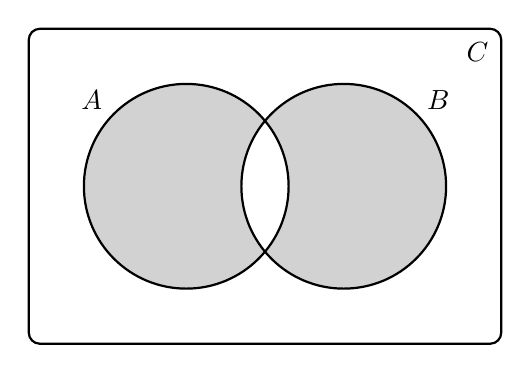
\begin{tikzpicture}

% Outer set C
\draw[thick, rounded corners] (-3,-2) rectangle (3,2);
\node at (2.7,1.7) {$C$};

% Shade A \ B
\begin{scope}
\clip (-1,0) circle (1.3cm);
\fill[gray!35] (-3,-2) rectangle (3,2);
\clip (1,0) circle (1.3cm);
\fill[white] (-3,-2) rectangle (3,2);
\end{scope}

% Shade B \ A
\begin{scope}
\clip (1,0) circle (1.3cm);
\fill[gray!35] (-3,-2) rectangle (3,2);
\clip (-1,0) circle (1.3cm);
\fill[white] (-3,-2) rectangle (3,2);
\end{scope}

% Sets A and B
\draw[thick] (-1,0) circle (1.3cm);
\draw[thick] (1,0) circle (1.3cm);

% Labels
\node at (-2.2,1.1) {$A$};
\node at (2.2,1.1) {$B$};

\end{tikzpicture}
\end{figure}
